\documentclass[tikz,border=7pt]{standalone}
% Shared TikZ style for the Nios V stereo accelerator diagrams.
\usepackage[T1]{fontenc}
\usepackage{lmodern}
\usepackage{xcolor}
\usepackage{tikz}
\usetikzlibrary{arrows.meta,backgrounds,calc,fit,positioning}

\definecolor{navy}{HTML}{073D73}
\definecolor{blue}{HTML}{0B5CAB}
\definecolor{cyan}{HTML}{1B8DBB}
\definecolor{green}{HTML}{27845B}
\definecolor{orange}{HTML}{C66A16}
\definecolor{red}{HTML}{B94444}
\definecolor{ink}{HTML}{172033}
\definecolor{muted}{HTML}{5A6678}
\definecolor{line}{HTML}{BFCBDA}
\definecolor{softblue}{HTML}{EDF4FA}
\definecolor{softcyan}{HTML}{ECF8FB}
\definecolor{softgreen}{HTML}{EEF8F2}
\definecolor{softorange}{HTML}{FFF4E8}
\definecolor{softgray}{HTML}{F5F7FA}

% Avoid automatic word hyphenation inside compact diagram nodes.
\hyphenpenalty=10000
\exhyphenpenalty=10000

\tikzset{
  font=\sffamily,
  block/.style={
    draw=line, rounded corners=2.2pt, fill=white,
    minimum height=10mm, text width=31mm, align=center,
    inner xsep=3mm, inner ysep=2.2mm
  },
  cpu/.style={block, draw=blue!55, fill=softblue},
  accel/.style={block, draw=cyan!65, fill=softcyan},
  memory/.style={block, draw=green!60, fill=softgreen},
  control/.style={block, draw=orange!65, fill=softorange},
  smallblock/.style={block, text width=24mm, minimum height=8mm, inner xsep=2mm, inner ysep=1.6mm},
  group/.style={draw=line, rounded corners=4pt, fill=softgray, inner sep=4mm},
  labeltag/.style={rounded corners=2pt, fill=navy, text=white, font=\sffamily\bfseries\footnotesize, inner xsep=2.5mm, inner ysep=1.2mm},
  flow/.style={-{Stealth[length=2.6mm,width=1.8mm]}, draw=navy, line width=0.85pt},
  dataflow/.style={-{Stealth[length=2.8mm,width=2mm]}, draw=blue, line width=1.15pt},
  controlflow/.style={-{Stealth[length=2.4mm,width=1.7mm]}, draw=orange, line width=0.9pt, dashed},
  returnflow/.style={-{Stealth[length=2.4mm,width=1.7mm]}, draw=green, line width=0.9pt},
  bus/.style={<->, >={Stealth[length=2.8mm,width=2mm]}, draw=navy, line width=1.6pt},
  note/.style={font=\sffamily\footnotesize, text=muted, align=left},
  arrowlabel/.style={font=\sffamily\scriptsize, text=muted, fill=white, inner sep=1.2pt}
}


\begin{document}
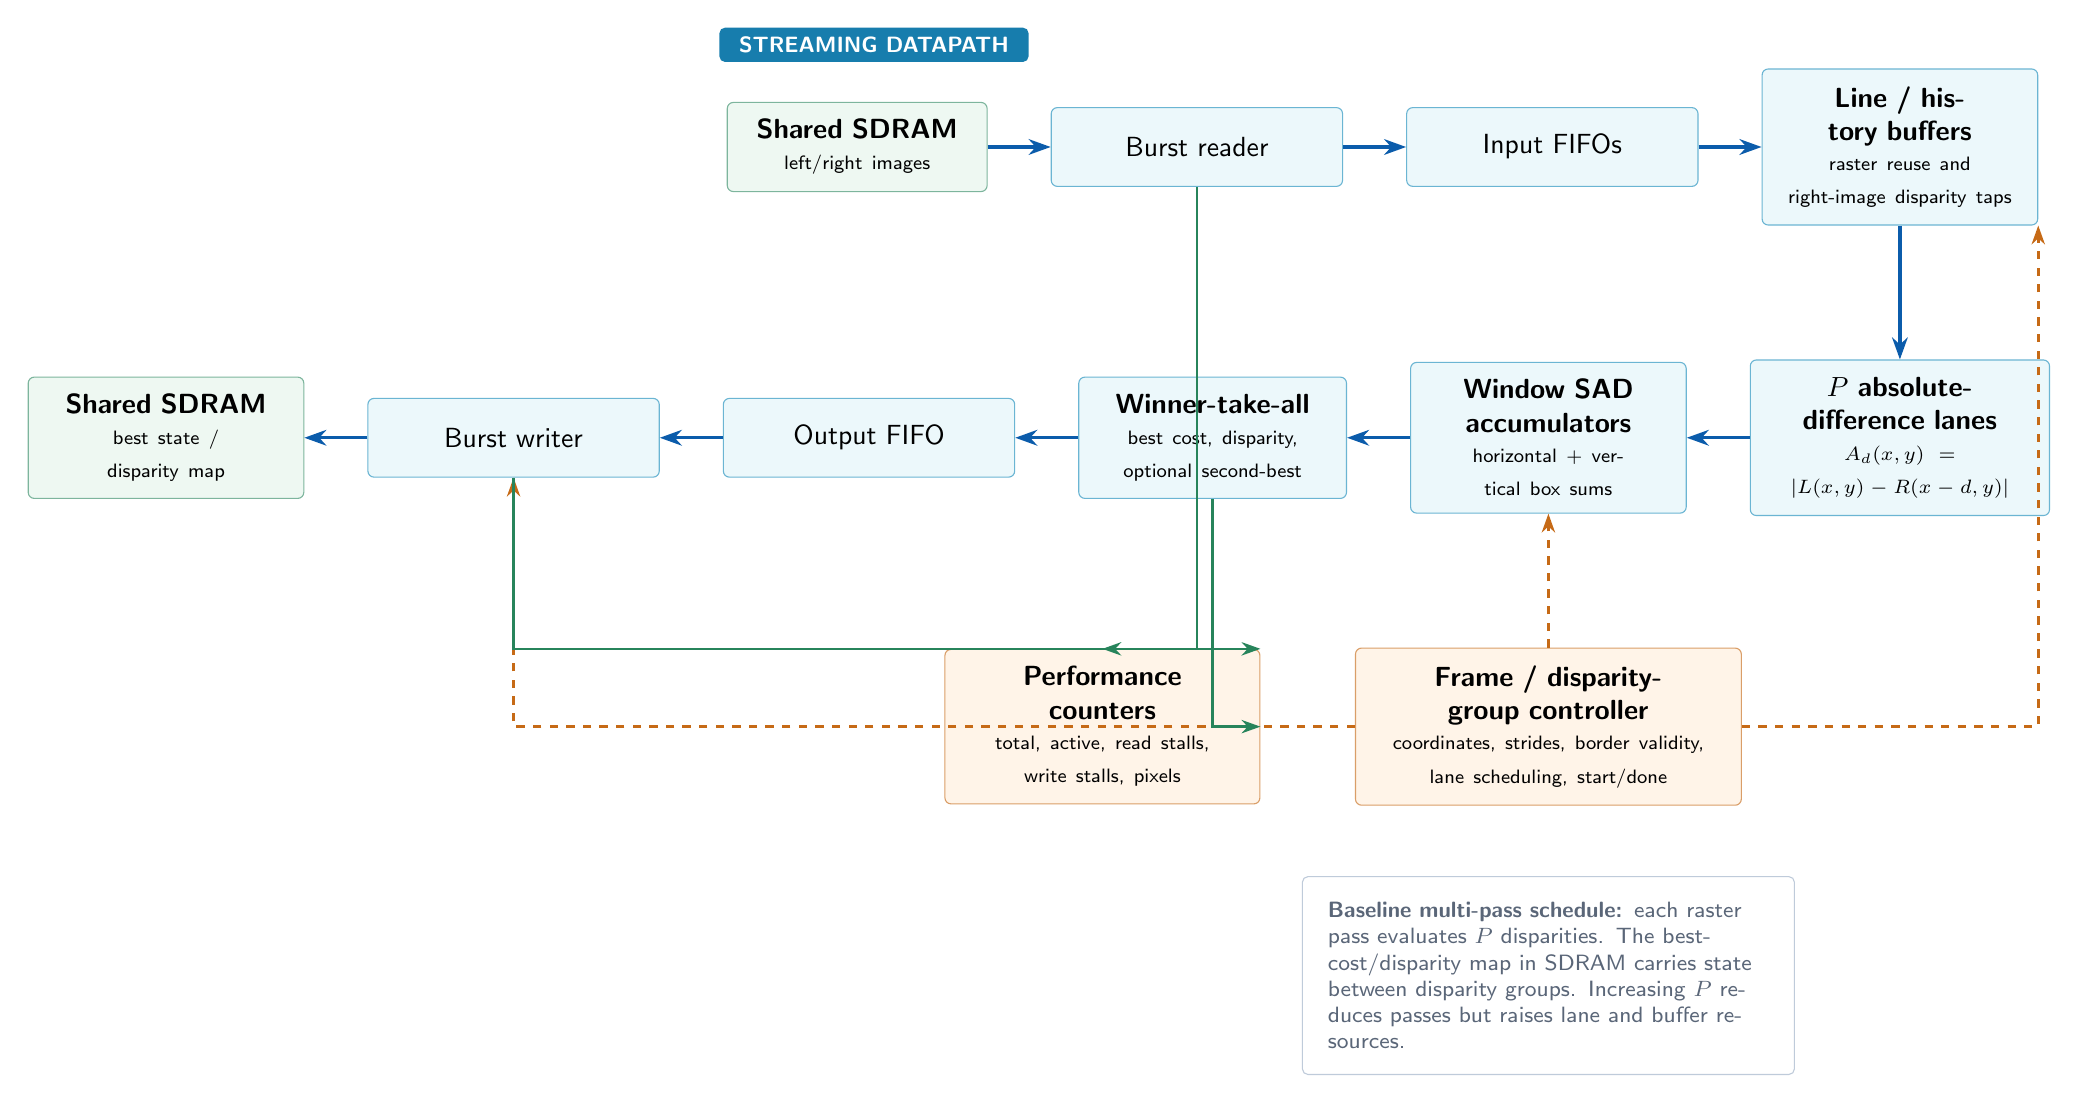
\begin{tikzpicture}[node distance=8mm and 8mm]
  \node[memory, text width=27mm] (sdramIn) {\textbf{Shared SDRAM}\\[-1pt]\scriptsize left/right images};
  \node[smallblock, accel, right=of sdramIn] (reader) {Burst reader};
  \node[smallblock, accel, right=of reader] (fifoIn) {Input FIFOs};
  \node[accel, text width=29mm, right=of fifoIn] (history) {\textbf{Line / history buffers}\\[-1pt]\scriptsize raster reuse and right-image disparity taps};

  \node[accel, text width=32mm, below=17mm of history] (abs) {\textbf{$P$ absolute-difference lanes}\\[-1pt]\scriptsize $A_d(x,y)=|L(x,y)-R(x-d,y)|$};
  \node[accel, text width=29mm, left=of abs] (box) {\textbf{Window SAD accumulators}\\[-1pt]\scriptsize horizontal + vertical box sums};
  \node[accel, text width=28mm, left=of box] (wta) {\textbf{Winner-take-all}\\[-1pt]\scriptsize best cost, disparity, optional second-best};
  \node[smallblock, accel, left=of wta] (fifoOut) {Output FIFO};
  \node[smallblock, accel, left=of fifoOut] (writer) {Burst writer};
  \node[memory, text width=29mm, left=of writer] (sdramOut) {\textbf{Shared SDRAM}\\[-1pt]\scriptsize best state / disparity map};

  \draw[dataflow] (sdramIn) -- (reader);
  \draw[dataflow] (reader) -- (fifoIn);
  \draw[dataflow] (fifoIn) -- (history);
  \draw[dataflow] (history.south) -- (abs.north);
  \draw[dataflow] (abs) -- (box);
  \draw[dataflow] (box) -- (wta);
  \draw[dataflow] (wta) -- (fifoOut);
  \draw[dataflow] (fifoOut) -- (writer);
  \draw[dataflow] (writer) -- (sdramOut);

  \node[control, text width=43mm, below=17mm of box] (controller) {\textbf{Frame / disparity-group controller}\\[-1pt]\scriptsize coordinates, strides, border validity, lane scheduling, start/done};
  \node[control, text width=34mm, left=12mm of controller] (counters) {\textbf{Performance counters}\\[-1pt]\scriptsize total, active, read stalls, write stalls, pixels};

  \draw[controlflow] (controller.north) -- (box.south);
  \draw[controlflow] (controller.east) -| (history.south east);
  \draw[controlflow] (controller.west) -| (writer.south);
  \draw[returnflow] (reader.south) |- (counters.north);
  \draw[returnflow] (writer.south) |- (counters.north east);
  \draw[returnflow] (wta.south) |- (counters.east);

  \node[note, text width=56mm, below=11mm of controller] (passnote) {\textbf{Baseline multi-pass schedule:} each raster pass evaluates $P$ disparities. The best-cost/disparity map in SDRAM carries state between disparity groups. Increasing $P$ reduces passes but raises lane and buffer resources.};
  \draw[draw=line, rounded corners=2pt] ([xshift=-2mm,yshift=-2mm]passnote.south west) rectangle ([xshift=2mm,yshift=2mm]passnote.north east);

  \node[labeltag, anchor=south west, fill=cyan!80!navy] at ([xshift=-1mm,yshift=5mm]sdramIn.north west) {STREAMING DATAPATH};
\end{tikzpicture}
\end{document}
